\section{Theory}\label{sec:theory}

This section will briefly explain the theory behind the genetic algorithm. It is defined as randomized, population based global search algorithm that tries to find global maximums or minimums of a certain function $f(x)$, in our case the Rosenbrock function: $$f(x,y) = (a-x)^2+b(y-x^2)^2$$, where $a$ and $b$ are parameters that define the function and $x$ and $y$ its coefficients. We start with an initial population $P(0)$ in which $x$ and $y$ are given as chromosomes (binary strings) of a certain size and evaluate the objective function (Rosenbrock) at points in $P(0)$ to get a fitness $F_{i}$ for each chromosome. The fitness represent a chromosome's score on the function, as a high value means we are close to either a global optimum or minimum. We save the fitness as the best-so-far chromosome and continue to create population $P_(1)$ from $P_(0)$ using the chromosomes with the best fitness so far, evaluate its fitness and so forth in an iterative manner. Given iteration $k=0$ and a initial population $P(0)$, the algorithm can be defined as\cite{Chong}:

\begin{itemize}
	\item 1. Evaluate $P(k)$. If stopping criterion is met, then stop.
	\item 2. Select $M(k) from P(k)$ as the mating pool.
	\item 3. Create new chromosomes from mating pool $M(k)$ by crossover and mutation.
	\item 4. Increase k by one and start over.
\end{itemize}

An interesting aspect is the crossover and mutation part, where we create new chromosomes (children) from binary strings (parents) with the best fitness of a population and mutate them afterwards. Figure \ref{fig:geneticalgocrossover} shows an example of a crossing, where the bit set of two parents are mixed at crossing sites to form two children. The crossing sites are chosen at random. Given two bit strings $0000$ and $1111{\color{red}4}$, the shown mutation would form two children $1100$ and $0011$. What follows is a mutation operation, where we flip bits in the children's bit string with a given probability $p_{m}$, usually a small value ($p_{m} < 0.01$), so only few chromosomes will be mutated. The idea behind these random crossings and mutations is that we seek a global maximum or minimum of our function $f(x)$ anywhere in the search space by avoiding getting stuck in local maximums or minimums, as is the case with gradient search methods. The particle swarm algorithm (PSO) shares similar attributes with genetic optimization.

\begin{figure}[h]
	\centering
	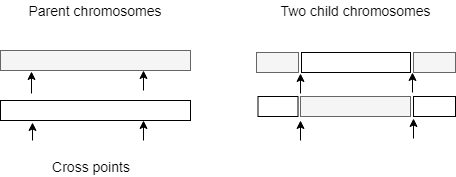
\includegraphics[width=0.7\linewidth]{theory/GeneticAlgoCrossover.png}
	\caption{An example of two parent chromosomes being crossed to create two children.}
	\label{fig:geneticalgocrossover}
\end{figure}

